Midterm logistics---we'll have the midterm Friday, during the regular section time. There will be 3-4 questions, of which we will choose a few and solve them in class. The full exam will then become a take-home which we'll work on over the weekend. Content runs through the Laplace chapter and not the Poisson chapter. In-class and take-home portions will be equally weighted (50/50).

\subsection*{Poisson's equation}
Laplace's equation is a special case of Poisson's equation. That is, Poisson's equation reads
\begin{equation}
    \nabla^2 \varphi = -\frac{\rho}{\epsilon_0}
\end{equation}
for vacuum or electric fields in (not-dielectric) matter, while
\begin{equation}
    \nabla^2 \varphi = -\frac{\rho_f}{\epsilon}
\end{equation}
in matter, where $\epsilon$ is the permittivity. This latter form is sometimes nice when we know the free charge.

A useful technique for solving boundary value problems in electrostatics is the \term{method of images}. We'll start with the classic example, a charge above a grounded plane.

\begin{exm}
    Suppose we have some charge $q$ a distance $z_0>0$ above a grounded conducting plane, $\varphi=0$. The method of images says that we can solve potential boundary value problems by matching the potential with an equivalent fictitious charge distribution.
    
    Notice that we can produce this same potential in the $z>0$ half-space if we place an ``image charge'' at $-z_0$. The potential from this distribution is
    \begin{equation}
        \varphi(x,y,z) = \frac{q}{4\pi \epsilon_0} \bkt{\frac{1}{\sqrt{x^2+y^2+(z-z_0)^2}} - \frac{1}{\sqrt{x^2+y^2+(z+z_0)^2}}}.
    \end{equation}
    The first term is the Poisson solution corresponding to our real charge, while the second term solves Poisson's equation in the upper half-space, so this will overall satisfy Poisson's equation for the \emph{real} charge distribution in the space we care about.
    
    One can easily check that on the plane $z=0$, we have $\varphi(x,y,0) =0$, so the boundary condition is satisfied.
    
    Notice that the potential from the plane below it ($z<0$) is its potential above, up to a $z\to -z$. That is,
    \begin{equation}
        \varphi_\text{plane} (x,y,z<0) = -\frac{q}{4\pi \epsilon_0 \sqrt{x^2+y^2 + (-z+z_0)^2}}.
    \end{equation}
    But that tells us that
    \begin{equation}
        \varphi_\text{plane} + \varphi_\text{charge} = 0 \text{ for } z<0,
    \end{equation}
    which we expected. The conductor has screened out the influence of the charge in the lower half-space.
    
    We can calculate the energy of this configuration by taking%
        \footnote{I did this a little differently from lecture. This is the field of two point charges separated by a distance $2z$.}
    \begin{equation}
        q\int_{z_0}^\infty dz\, E(z) = \int_{z_0}^\infty dz \frac{q^2}{4\pi \epsilon_0 (2z)^2} = \frac{q^2}{4\pi \epsilon_0} \paren{-\frac{1}{4z_0}}.
    \end{equation}
    
    Equivalently this is half of the interaction energy of the charge and the image charge; we can see this by integrating over the energy in the field of two real charges and then arguing by symmetry that we only have field in the half-space, so the actual energy is half the energy of the real dipole.
    
    We can now calculate the charge distribution by looking at the normal derivative of potential at the conductor. Here,
    \begin{equation}
        -\P{\varphi}{z}|_{z=0^+} = \frac{\sigma}{\epsilon_0}.
    \end{equation}
    We have
    \begin{equation}
        \sigma/\epsilon_0 = \frac{q}{4\pi} \bkt{-\frac{z_0}{(\rho^2 + z_0^2)^{3/2}} - \frac{z_0}{(\rho^2+z_0^2)^{3/2}}},
    \end{equation}
    so then the total induced charge is
    \begin{align*}
        Q &= \int_0^\infty (2\pi \rho d\rho) \sigma(\rho,\phi)\\
            &= \int_0^\infty (2\pi \rho d\rho) \frac{q}{4\pi} \bkt{-\frac{z_0}{(\rho^2 + z_0^2)^{3/2}} - \frac{z_0}{(\rho^2+z_0^2)^{3/2}}}\\
            &= -q \int_0^\infty d\rho \frac{\rho z_0}{(\rho^2 +z_0^2)^{3/2}}\\
            &= \frac{q z_0}{(\rho^2+ z_0^2)^{1/2}}|_0^\infty\\
            &= -q.
    \end{align*}
    We learn that the induced charge was exactly equal and opposite to the real charge, as we might have guessed.
\end{exm}

\begin{exm}
    Let us now revisit a situation we've considered before. We have a charge $+q$ embedded in some dielectric of dielectric constant $\kappa_L$ which fills the region $z<0$, a distance $d$ from the interface with a different dielectric $\kappa_R$ which fills $z>0$.
    
    Emboldened by our success with the conducting plane, we might think that perhaps an image charge approach could work for the interface between dielectrics as well. That is, let's cook up a scenario where there's some image charge $q_R$ in a dielectric $\kappa_L$ on the right. It doesn't matter that the image charge configuration has $\kappa_L$ on the right now, since we just want to fit the boundary conditions at $z=0$.
    
    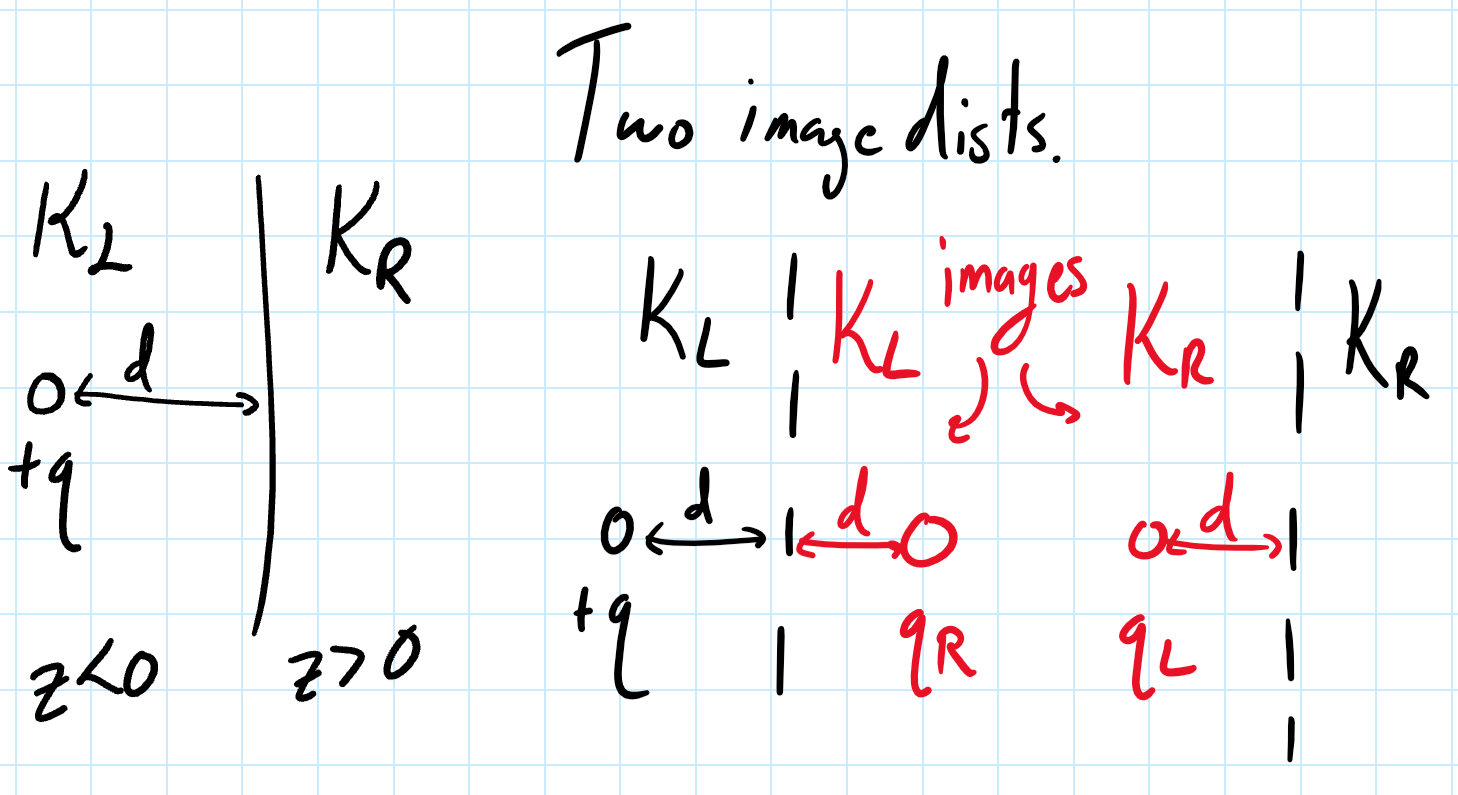
\includegraphics[width=0.95\textwidth]{2020/02/20200204_dielectric_images}
    
    It follows that the potentials in each region are
    \begin{gather}
        \varphi_L(x,y,z) = \frac{1}{4\pi \epsilon_L} \bkt{\frac{q}{\sqrt{x^2+y^2+(z+d)^2}} + \frac{q_R}{\sqrt{x^2+y^2+(z-d)^2}}},\\
        \varphi_R (x,y,z) = \frac{1}{4\pi\epsilon_R} \frac{q_L}{\sqrt{x^2+y^2+(z+d)^2}}.
    \end{gather}
    %
    The potential is continuous,
    \begin{equation}
        \varphi_L(x,y,0) = \varphi_R(x,y,0),
    \end{equation}
    while its normal derivative is discontinuous,
    \begin{equation}
        \kappa_L \epsilon_0 \P{\varphi_L}{z}|_z=0 = \kappa_R \P{\varphi_R}{z}|_{z=0}.
    \end{equation}
    Continuity tells us that
    \begin{equation}
        \frac{q+q_R}{\kappa_L} = \frac{q_L}{\kappa_R},
    \end{equation}
    and the normal derivative gives the condition that
    \begin{equation}
        -q d + q_R d = -q_L d.
    \end{equation}
    That is,
    \begin{equation}
        q=q_R + q_L.
    \end{equation}
    We now have two equations relating $q,q_R,$ and $q_L$, which we can easily solve
    \begin{equation}
        q_L = \frac{2\kappa_R}{\kappa_R + \kappa_L}q, \quad q_R = \frac{\kappa_L-\kappa_R}{\kappa_L + \kappa_R}q.
    \end{equation}
    We can then check that for $\kappa_L=\kappa_R$, we have $q_R=0$ and $q_L=q$. This says there's no image charge on the right (there's no boundary) and our left image charge is just the original charge.
\end{exm}

Like in Gauss's law, image charges only really work when we have a large amount of symmetry.